\chapter{Discussion and Analysis}
\label{ch:evaluation}
\section{Significance of the Findings}
The results from the regression models show that using machine learning is really helpful for predicting forest fires. Even though it's a tough problem, these models can make good predictions when we get the data ready properly. By looking at past weather, geography, and fire data, these models can find patterns that help predict fires. This helps us get ready for fires and manage them better.

\section{Performance Analysis}
Among the models we looked at, CatBoost did the best at predicting fires. It's really good at handling different types of data and finding tricky patterns. XGBoost and LightGBM also did well, but CatBoost was a bit better. These models are good at handling lots of data and figuring out what's important for predicting fires

\begin{figure}[ht]
    \centering
    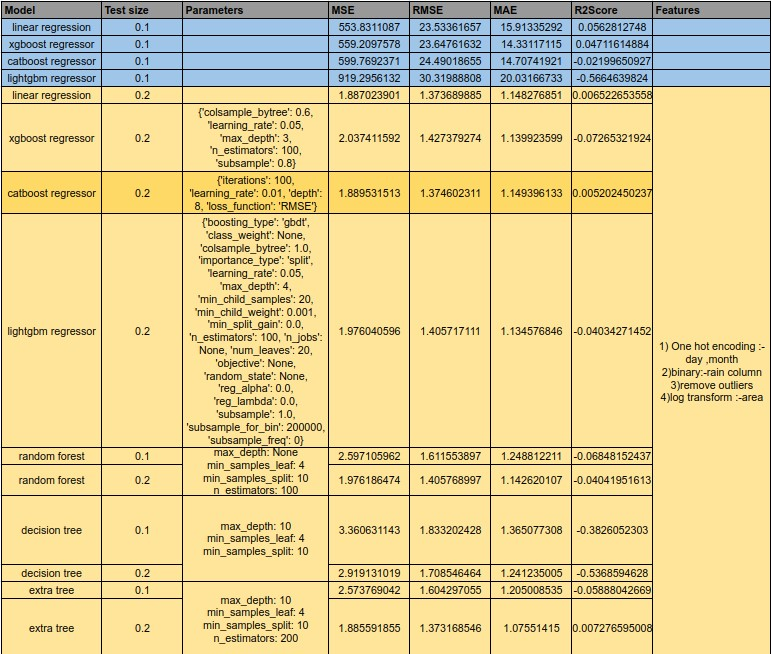
\includegraphics[scale=0.8]{figures/Comprehensive overview of various model configurations.jpg}
    \caption{Table 4: This table presents a comprehensive overview of various model configurations, including hyperparameters and corresponding evaluation metrics.}
    \label{fig:example-02}
\end{figure}

Additionally, an extra feature was integrated into the project to predict fire severity into three categories: mild, moderate, and severe. This enhancement offers more nuanced insights into the potential severity of forest fires, enabling better preparation and management strategies. By incorporating this additional feature, the models can anticipate the intensity of fire outbreaks more accurately and assist in effective resource allocation and mitigation efforts.

\section{Limitations and Implications}

However, it's essential to acknowledge several limitations inherent in the analysis. The performance of the models is heavily reliant on the quality and representativeness of the dataset. Inadequate or biased data can lead to erroneous conclusions and hinder the generalizability of the models. Moreover, the choice of hyperparameters and preprocessing techniques can significantly impact model performance, highlighting the importance of thorough experimentation and tuning.

Additionally, the scarcity of certain data points within the dataset poses challenges for model training and evaluation. Variables with limited observations or missing values may not adequately represent the underlying distribution of data, potentially leading to biased predictions. Addressing these data deficiencies requires innovative approaches such as data imputation techniques or the integration of supplementary data sources.


\section{Summary}

In summary, the findings from the regression models demonstrate the potential of machine learning in forest fire prediction. By optimizing model performance and addressing data limitations, we can enhance the reliability and robustness of predictive models for effective forest fire management. Ongoing research efforts are crucial for advancing our understanding of forest fire dynamics and improving prediction accuracy in real-world scenarios.